\section{球密度による影響}

超音波照射された擬塑性流体中に球を落下させた結果をFig.\ref{fig:0.05-0.2}-\ref{fig:1.5}に示す.この結果より,濃度ごとに終端速度を求めた結果をFig.\ref{fig:rhoUT}に示す.縦軸は終端速度$U_\text{T}$,横軸は密度差$\Delta\rho$である.密度差が大きくなると,終端速度が大きくなることが分かった.また,濃度ごとに高速化度合を求めた結果をFig.\ref{fig:rhoUdiff}に示す.縦軸は高速化度合$U_\text{on}/U_\text{off}$,横軸は密度差である.PAA濃度0.2,1.5wt.\%においてはあまり高速化が見られなかった.一方で,0.5,1.0wt.\%において,密度差が小さくなると高速化が顕著にみられた.

超音波照射された擬塑性流体中を落下する球の高速化に対する,落下球の密度による影響を考える.\ref{sec:UTdiff}節にて示した,落下球の高速化度合の理論式(\ref{eq:Udiff})に終端速度の理論式(\ref{eq:UT})を代入すると,
\begin{eqnarray}
    \frac{U_{ABL}}{U_T} \sim \left(\frac{\Delta\rho{}g}{3}\right)^{\frac{n-1}{n}}\cdot\frac{2-n}{n}\cdot\frac{\delta}{\mu_{ABL}}\cdot\left(\frac{k}{a}\right)^{\frac{1}{n}} ,
    \label{eq:UdiffRho}
\end{eqnarray}
となる.本実験において,落下球の密度をパラメータとして考える.他の条件に関して同一であると考えると,超音波照射に伴う高速化は式(\ref{eq:UdiffRho})より,
\begin{eqnarray}
    \frac{U_{ABL}}{U_T} \sim \left(\Delta\rho{}\right)^{\frac{n-1}{n}} ,
    \label{eq:UdiffRho2}
\end{eqnarray}
と表される.

これらの結果より式(\ref{eq:UdiffRho2})を用いて,落下球と流体の密度差と,超音波照射による高速化の関係性をFig.\ref{fig:rhoUdiffAll}に示す.縦軸は高速化度合$U_\text{on}/U_\text{off}$,横軸は密度差のみによる影響を考慮した$\Delta\rho^{\left(\left(n-1\right)/n\right)}$である.全条件の結果をFig.\ref{fig:rhoUdiffAll}(a)に,0.2wt.\% PAA溶液以外の結果をFig.\ref{fig:rhoUdiffAll}(b)に示す.0.2wt\%PAA溶液の条件において,高速化度合は密度差のみによる影響に対して,相関関係は見られなかった.これは,0.2wt\%PAA溶液においてPAA濃度が非常に希薄であるため,高速化現象が発生していないためだと考えられる.一方でそれ以外の条件において,高速化度合は密度差のみによる影響に対して弱い正の相関関係を示した.これは,密度差以外の濃度による影響を考慮していないためだと考えられる.このことより,密度差を用いて超音波照射された擬塑性流体中を落下する球の高速化度合を整理することができることが分かった.

\begin{figure}[ht]
    \centering
    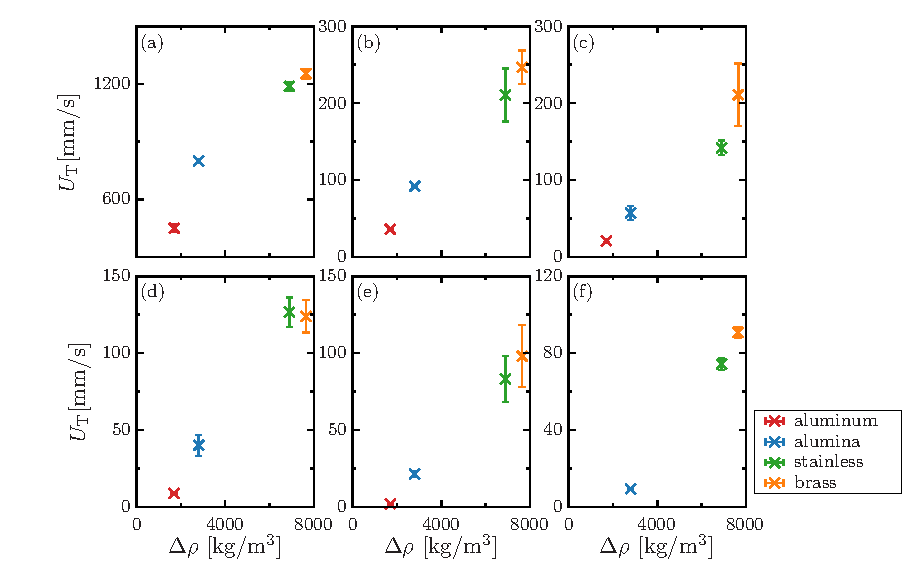
\includegraphics[width=1.0\textwidth]{./5-Results/rhoUT.eps}
    \caption{Termination velocity by density difference in PAA solution (a)0.2wt.\%, (b)0.5wt.\%, (c)0.7wt.\%, (d)1.0wt.\%, (e)1.3wt.\%, (f)1.5wt.\%.}
    \label{fig:rhoUT}
\end{figure}

\begin{figure}[ht]
    \centering
    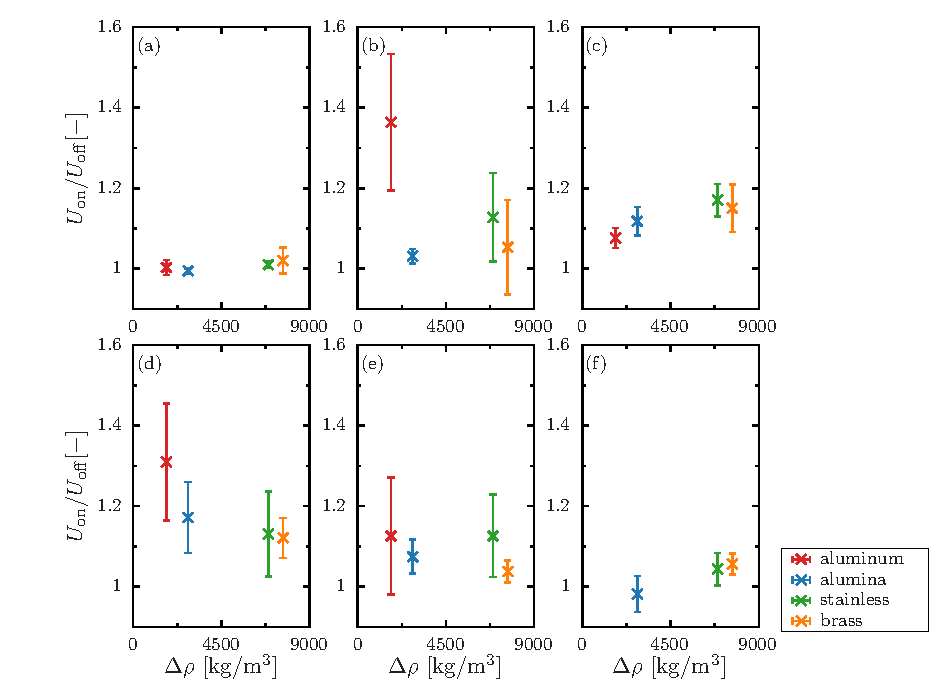
\includegraphics[width=1.0\textwidth]{./5-Results/rhoUdiff.eps}
    \caption{Velocity ratio by density difference in PAA solution (a)0.2wt.\%, (b)0.5wt.\%, (c)0.7wt.\%, (d)1.0wt.\%, (e)1.3wt.\%, (f)1.5wt.\%.}
    \label{fig:rhoUdiff}
\end{figure}

\begin{figure}[ht]
    \centering
    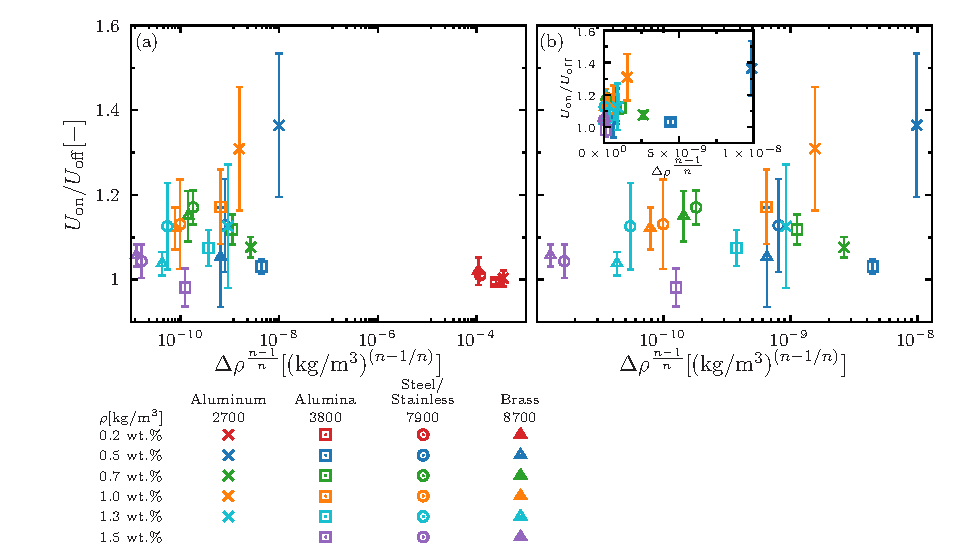
\includegraphics[width=1.0\textwidth]{./5-Results/rhoUdiffAll.eps}
    \caption{Relationship between density difference and velocity ratio by (a)all data, (b)with out 0.2wt.\% PAA solution data.}
    \label{fig:rhoUdiffAll}
\end{figure}